\chapter{Approach}

\section{System context}

The reimbursement-tool interacts with multiple actors and other software interfaces. In this section those interactions will be defined in detail.

\subsection{Context diagram}

The context diagram (see figure \ref{fig:context-diagram}) describes the important relationships between the system and its interrogators. \textit{Expense creator} such as normal employees or even professors can create expenses and print them. However, they are not allowed to modify an expense if it's not in draft state anymore. Further only the \textit{Managers} and the \textit{Finance admins} are allowed to \textit{Reject expenses} back to the \textit{Expense creator}. Besides rejecting, they are also allowed to modify expenses after it has been submitted by the \textit{Expense creator}.\newline
\textit{Guests} are allowed to view specific expenses. However, they need the 32-character long internal expense \textit{Uid} to gain access to it. The \textit{Uid} is added on the printed expense document. All other interrogators have access to all expenses they have to work with.\newline
The following sub chapters will explain why the interfaces to external service providers are necessary.

\subsubsection{UZH LDAP Server}

The system fetches the user data from the UZH-IFI LDAP server (see figure \ref{fig:context-diagram}). This is necessary to synchronize the user database, to allow all registered users at the IFI LDAP use the system without creating a new user name and password to access the systems functionality. Currently the synchronisation interval is defined to take part every 300 Seconds. By changing the 
value of \textit{reimbursement.ldap.refreshRate} on the file \textit{application.properties} stored at the 
back-end in the directory \textit{src/main/resources}. 


\begin{figure}[H]
    \centering
    \fbox{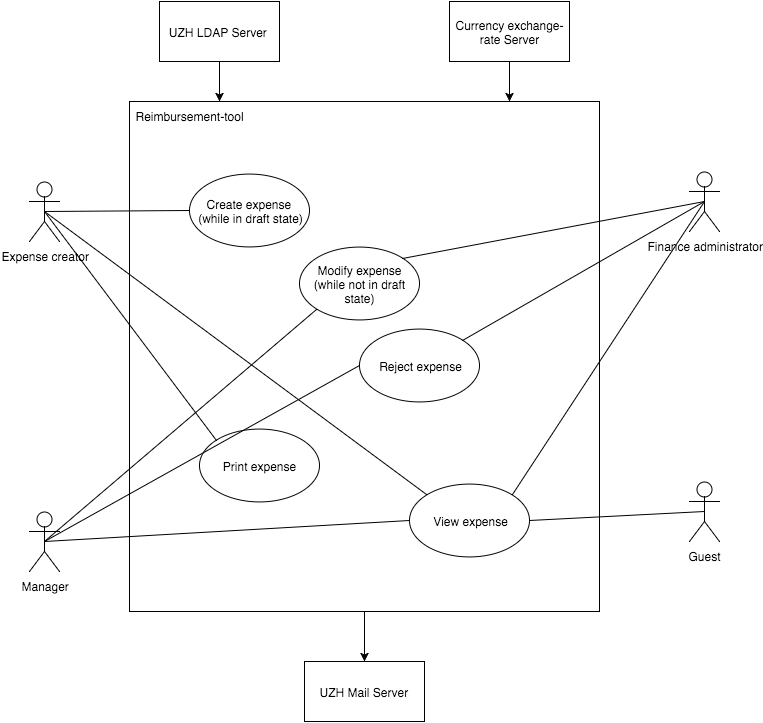
\includegraphics[width=0.80\textwidth]{context-diagram}}
    \caption{System context: Context diagram}
    \label{fig:context-diagram}
\end{figure}

\subsubsection{Currency exchange-rate Server}

To support the reimbursement-tool with accurate currency exchange-rates it needs to access an external API that provides that data. We used \url{fixer.io} \cite{fixer} because it's free,  it's updated daily, has a high responsibility and high availability rate. Currently the reimbursement-tool calls the API every time an exchange-rate is needed. 

\subsubsection{UZH Mail Server}

To notify participants about outstanding expense and actions that need attention, it is necessary to add a mailing service. Therefor the reimbursement-tool needs to have access to the UZH Mail Server.\newline
The currently used e-mail header settings can be adjusted at the \textit{application.properties} file in the back-end.\newpage



\section{Architecture}

The back-end is considered as the software and database that runs on a Tomcat \cite{tomcat} server and a PostgreSQL \cite{postgresql} for the database. The system is hosted by the IFI \cite{ifi}. The front-end/client communicates with the back-end using RESTful services described in section \ref{sec:restfulapi}.

\subsection{Back-end}
The back-end is developed in Java. It is structured according to the rules of Domain Driven Design (DDD) \cite{ddd}. The domain model, that consists of the concepts, is connected to the database. Changes on the model will be automatically synchronized with the database. The service package lists all methods for a specific domain model.\newline DTOs (Data Transfer Object) are used to transfers data from back-end to front-end and vice verse. \newline The implemented model- and service-classes are visualized in the appendix \ref{sec:app-models} and \ref{sec:app-service}  

\subsection{Front-end}
The front-end is developed in JavaScript using the AngularJS \cite{angular} framework. Angular is based on an MVC (Model View Controller) pattern. It basically consists out of controllers, templates used for the view, as well as models that are shown to the user using the templates. However, AngularJS \cite{angular} extends the basic pattern with many useful concepts like directives, filters, injectors etc. A complete list of the vailable concepts in AngularJS and small examples can be found at the AgngularJS: Developer Guide \cite{angular-devguide}.   

\subsection{Multilayer architecture}
We use a common \textit{Multilayer architecture} (see figure \ref{fig:architecture-layer}) in the back-end to provide a good overview of the entire software-code. The following four layers are used:
\begin{itemize}
    \item \textbf{Presentation Layer} provides the front-end code for the GUI creation. It uses \textit{AngularJS} for the GUI creation. The \textit{Presentation Layer} interacts with the \textit{Application Layer}.
    \item \textbf{Application Layer} provides the available services that interact with the \textit{Business Layer}. It hosts the Security, RESTful services and the Global Exceptions.
    \item \textbf{Business Layer} provides the available services that interact with the \textit{Data Access Layer}. It provides the relevant services and models based on the \textit{Data Access Layer}.
    \item \textbf{Data Access Layer} consists of repositories and the \textit{Hybernate} database. 
\end{itemize}

\begin{figure}[H]
    \centering
    \fbox{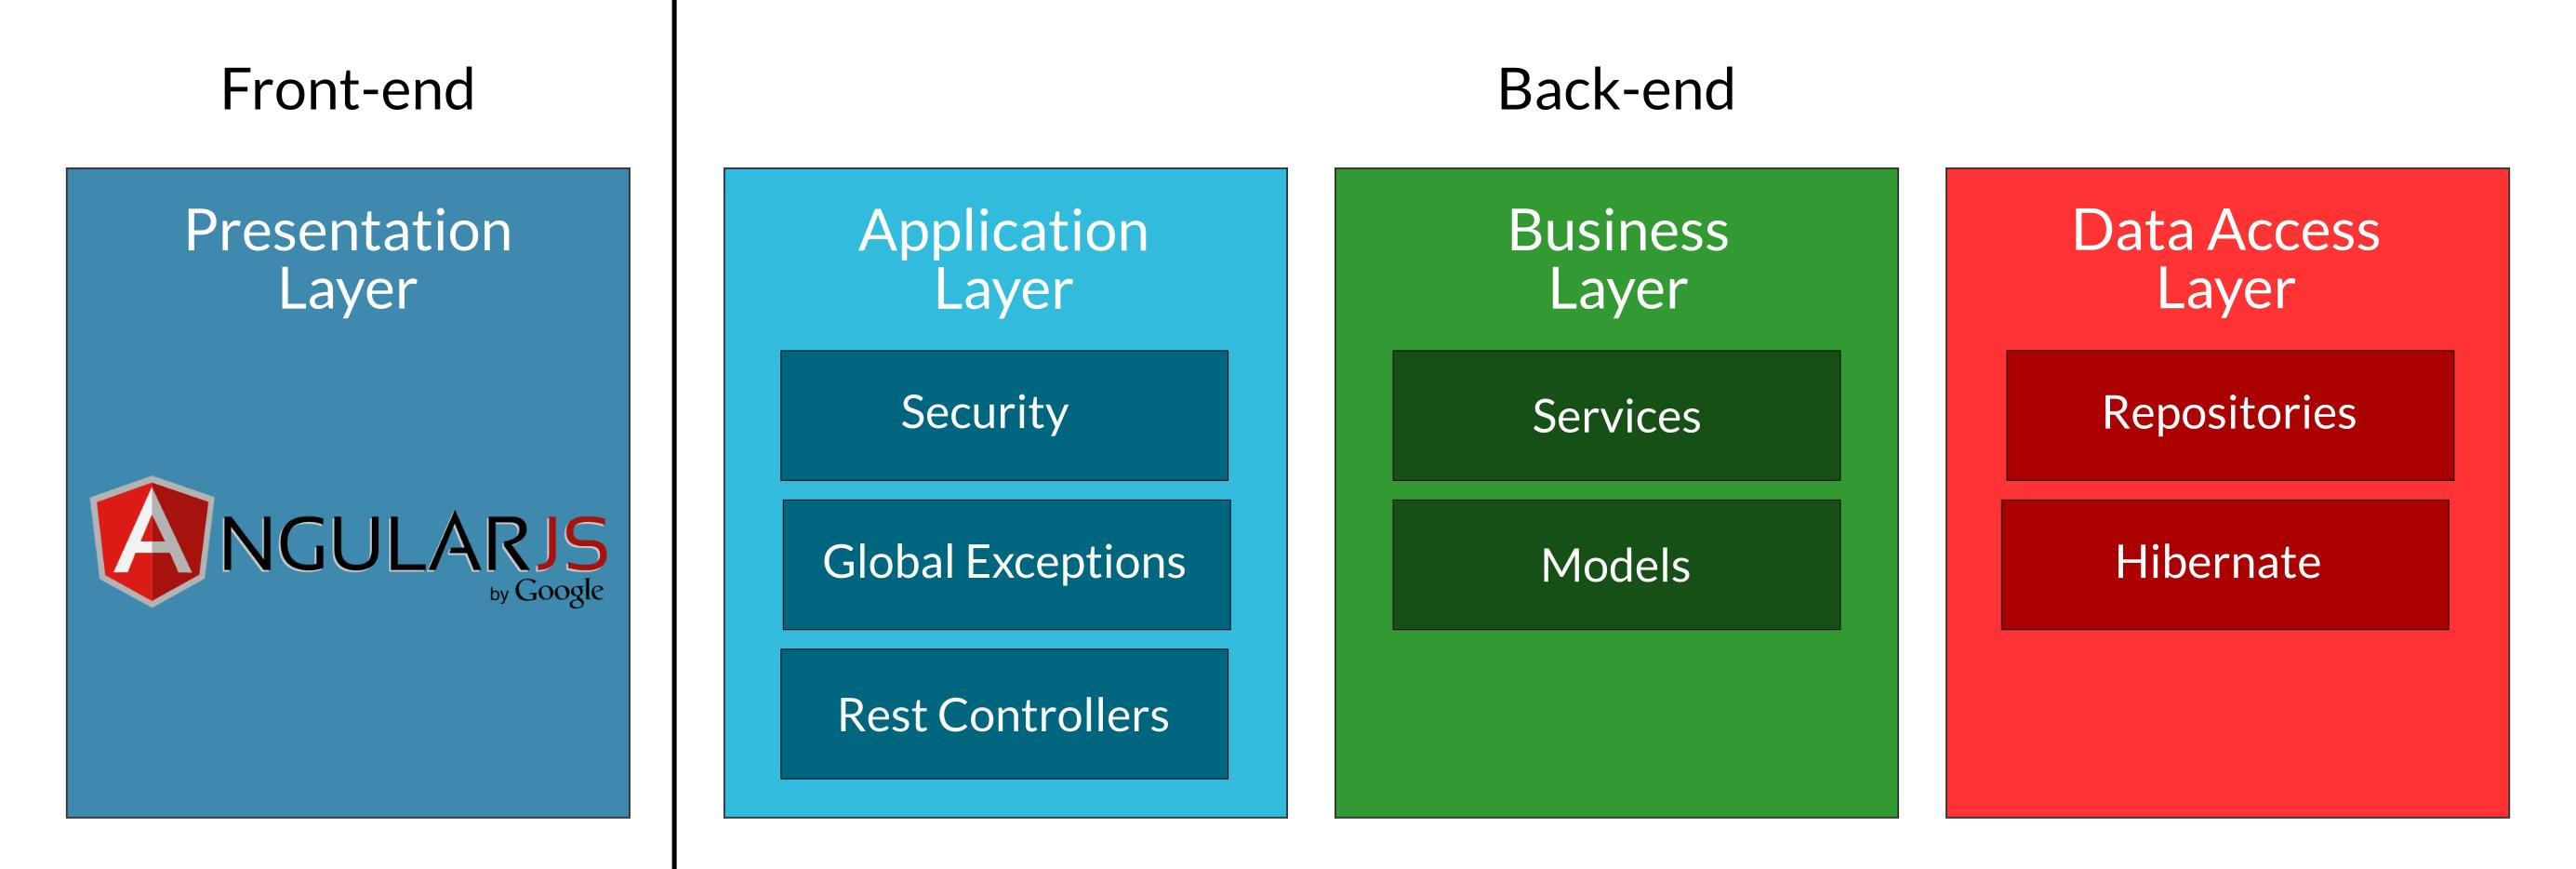
\includegraphics[width=0.80\textwidth]{architecture-layer}}
    \caption{Architecture: Multilayer architecture}
    \label{fig:architecture-layer}
\end{figure}

Our layers depend on each other while every layer communicates only with either the upper or the lower layer. This ensures a good maintainability and loose coupling of the single layers.\newline 
For example: If the presentation layer needs to display an expense, the application layer will handle this request by first checking the relevant security parameter of the request followed by calling the business layer. The service will handle and aggregate the desired information fetched from the relevant models. In our case to display an expense, the service will retrieve all expense-items and expense-item-attachments.


\section{Processflow}
\label{sec:processflow}
As described in \ref{sec:states} an expense always has to be in one specific state. The entire process implemented in the system is documented in the appendix \ref{sec:process-diagram-rotated}. The four lanes point out user roles.\newline 
The process starts in the lane \textit{Employee}; an expense is created, \textit{Receipts} are added and it is forwarded to the next higher instance for verification. After verifications by the \textit{Manager} or \textit{Department manager} and \textit{Finance administration} are successful, the signing will start. During the signing, all three entities; \textit{Employee}, \textit{Manager} and the \textit{Finance administration} needs to sign the document. If all of them have signed the document correctly, the creator - in our case the \textit{Employee} - can print the expense and hand it over over to the \textit{Finance administration}. Currently this process step is not integrated in best practice. Because all of the expense receipts will be printed and after verification of the \textit{Finance administration UZH} it they will be digitalized again. This media disruption is also described in section \ref{future-work} Future Work.

\subsection{States}
\label{sec:states}
During the process an expense passes through various states. The available user roles (see section \ref{user-roles}) have different authorizations to change the state of an expense.  

\begin{itemize}
    \item \textbf{DRAFT} state occurs if the expense is created and yet has not been assigned to a \textit{Manager}.
    
    \item \textbf{TO\_BE\_ASSIGNED} state occurs if the expense is submitted, but has not been assigned to a specific manager or finance admin. If the expense has been assigned, the expense will either have the state \textbf{ASSIGNED\_TO\_MANAGER} or \textbf{ASSIGNED\_TO\_FINANCE\_ADMIN}.
    
    \item \textbf{ASSIGNED\_TO\_MANAGER} state occurs if the expense is assigned to a specific \textit{Manager}.
    
    \item \textbf{ASSIGNED\_TO\_FINANCE\_ADMIN} state occurs if the expense is assigned to a specific \textit{Finance admin}.
    
    \item \textbf{REJECTED} state occurs if the created expense is not accepted by the \textit{Manager}, \textit{Department manager} or \textit{Finance management}. In \textbf{Rejected} status the expense will be reassigned to the user who created it.
    
    \item \textbf{SIGNED} state occurs if the expense has been signed by all participants; \textit{Registered user}, \textit{Manager} or \textit{Department manager} and \textit{Finance management}. There exist sub states that occur if the expense is in the process of being signed by all participants:
        \begin{itemize}
            \item \textbf{TO\_BE\_SIGNED\_BY\_USER} occurs if the expense needs to be signed by the \textit{User}.
            \item \textbf{TO\_BE\_SIGNED\_BY\_MANAGER} occurs if the expense needs to be signed by the \textit{Manager}.
            \item \textbf{TO\_BE\_SIGNED\_BY\_FINANCE\_ADMIN} occurs if the expense needs to be signed by the \textit{Finance admin}.
        \end{itemize}
    
    \item \textbf{PRINTED} state occurs if the expense and all its receipts are successfully converted into a digital document.
    
    \item \textbf{ARCHIVED} state occurs if the expense has been printed.
    
\end{itemize}

\subsection{E-mail notification}
To inform the users of the reimbursement-tool about changes, e-mail notifications had been implemented to update affected users immediately. Basically e-mail notifications are executed at the following actions:
\begin{itemize}
\item An Expense that has been created by a User and is assigned to a Manager, will execute an e-mail to the respective Manager.
\item An Expense that has been approved by the Manager and enters the state \newline \textbf{TO\_BE\_ASSIGNED}, will execute an e-mail to all available Finance admins.
\item An Expense that needs to go through the signing process, will execute an e-mail to notify every signing entity.
\item If an Expense is rejected by the Manager or Finance admin the User who created the Expense will receive an e-mail notification.
\end{itemize}

Besides state changes e-mails will also be sent to an administrator if a general run-time exception occurs. To ensure the administrator of the reimbursement-tool is up-to date about major incidents. Those kind of \textit{emergency e-mails} will only be sent, if if the exception is not a type of \textit{BusinessException} or \textit{AccessDeniedException}. 
    

\section{Technologies}

In the following section the technologies used on the reimbursement-tool are being described and if necessary, explained why they had been chosen. 

\subsection{Back-end}

\subsubsection{Java}
The reimbursement-tool uses Java SE 7 for the Back-end programming language. Java is an industry wide standard, has detailed documentation and sufficient knowledge at the IFI \cite{ifi} department to guarantee an adequate support and future development of the software.

\subsubsection{Hibernate}
Hibernate abstracts the data layer. So that SQL-queries have to be written in rare cases only, which increases the code-clarity and decreases the code-complexity which can lead to bugs and errors. All data operation are handled implicitly by defined Java data classes.\newline
H2 database is a temporary database for storing data in a database environment. It offers a simple interface and can be used for developing, if only one development server database is available. \cite{hibernate}

\subsubsection{Java Spring Framework}
The reimbursement-tool uses various services of the Java Spring Framework \cite{spring}:
\begin{itemize}
    \item Spring Security for the login- and user-management as well as role based access-management for the RESTful resources.
    \item Spring Web MVC framework used to define RESTful interface within a few lines of code.
    \item Spring ORM used for the XML mapping within the process of Pdf-generation.
    \item Spring data is used to provide a simpler method to use data access technologies. It uses the DAO (Data Access Object) \cite{dao} to access data in a standard database like SQL. 
\end{itemize}

\subsubsection{Maven}
The tool uses Apache Maven \cite{maven} for the build process and dependency management.  

\subsubsection{Mockito}
The tool uses the Mockito framework to mock services. It can be used to write tests with a clean and simple API. Further it's easy to integrate with the Java Spring Testing framework. \cite{mockito}

\subsubsection{FOP-Apache}
After the process completion, the captured expenses need to printed on two A4 pages in landscape format. The structure of the sheets are predefined by the university. The generated Pdf by the reimbursement-tool needs to be identical to the existing MS-Office Excel file. See appendix \ref{sec:app-pdf} for the generated Pdf structure.\newline
The Pdf get generated using an individual created XSLT template and a XML document generated out of a Java Object. Combining these two files generates an FO document, which will be used by Apache FOP \cite{apache-fop} to generate a Pdf.\newline
We decided for Apache FOP because it is based on widely used standards like XML and XSL so that ongoing maintenance can be easily and without specific knowledge achieved.

\subsection{Interface}

\subsubsection{RESTful API}
\label{sec:restfulapi}
The tool uses a RESTful API that provides methods to access the Backend resources. It is implemented using the Spring MVC. 

\subsubsection{Swagger UI}
The Swagger UI visualizes all methods provided by the REST interface within a GUI. Furthermore developers can interact directly with the interface to test the methods. figure \ref{fig:swagger01} shows a screenshot of our used Swagger interface. It visualizes all the available methods for the \texttt{public} resource as well as the mandatory and optional parameters for \texttt{HTTP} calls. This was important for the process of development. \cite{swagger}

\begin{figure}[H]
    \centering
    \fbox{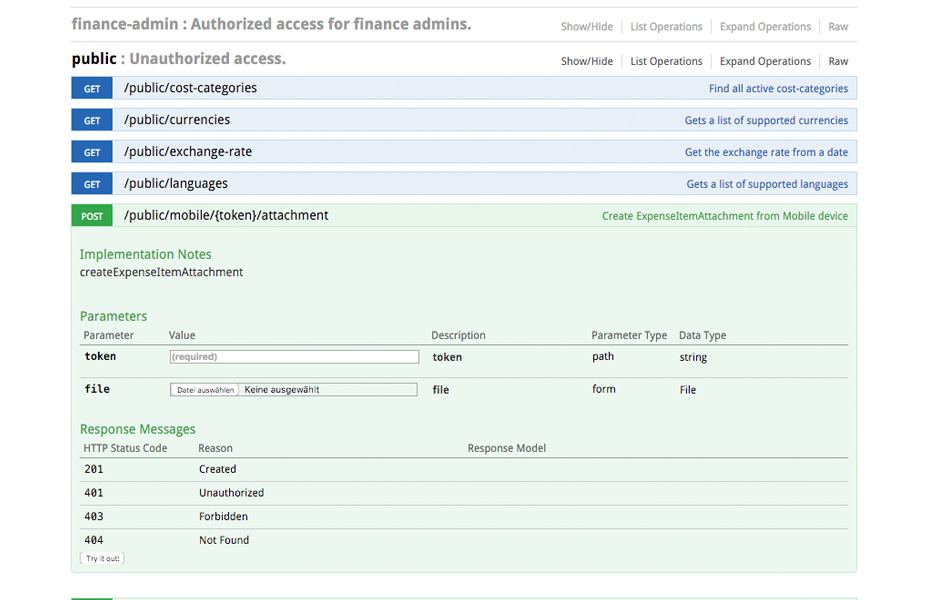
\includegraphics[width=0.80\textwidth]{swagger01}}
    \caption{Swagger: Reimbursement GUI}
    \label{fig:swagger01}
\end{figure}

\subsection{Front-end}

\subsubsection{AngularJS}
The tool uses the AngularJS framework for the client. Its data bindings and dependency injections reduces the amount of code need to be written. Further it uses HTML templates and a routing framework to create an interactive GUI. AngularJS is based on an MVC approach and is easy to integrate with REST services.\cite{angular}\par


\subsubsection{Bootstrap}
Bootstrap is a framework that consists of HTML, CSS and JavaScript elements that can be used to create appealing responsive websites. It is supported by most of the desktop and mobile web browsers available. The tool uses Bootstrap v. 3.3.5. \cite{bootstrap}

\subsubsection{Bower}
The tool uses Bower for the client-side package management. Bower is a package manager for JavaScript web applications like AngularJS. It keeps track of the used assets, frameworks, libraries, etc. \cite{bower}  

\subsubsection{Grunt}
Grunt is a JavaScript task runner. We use it for our client-side build. Its plugin directory supports a lot of modules to optimize the development work flow. Code-uglifying, concating, sass-compiling, file operations, auto prefixing etc. \cite{grunt} 
